\section{Illustrative Example}
    \normalsize 
    A one-dimensional example is used to demonstrate the performance of the crude Monte Carlo method and the importance sampling technique. This example perfectly exemplifies the rare-event situation in which high-consequence samples are located in low-probability regions. 
    In this example, $x$ is a continuous random vector, $f(x)$ is the scalar function of $x$ (or the model under study), and $p(x)$ is the probability density function of $x$, which are expressed as follows: 
    $$p(x)=\mathcal{N}(\mu,\,\sigma^{2})$$
    $$f(x)=\frac{1}{2} \Bigr[ 1+erf \Bigl( \frac{x-\mu}{\sqrt{2}\sigma} \Bigl) \Bigr] \quad \text{and} \quad erf(x)=\frac{2}{\sqrt{\pi}}\int_{0}^{x}exp(-t^2)dt$$
    where $\mu$ and $\sigma$ represent the mean and standard deviation of $x$, respectively. \\
    The $f(x)$ and $p(x)$ functions are depicted in Fig.~\ref{fig:f&p}.
    
        \begin{figure}[H]
        \centering
        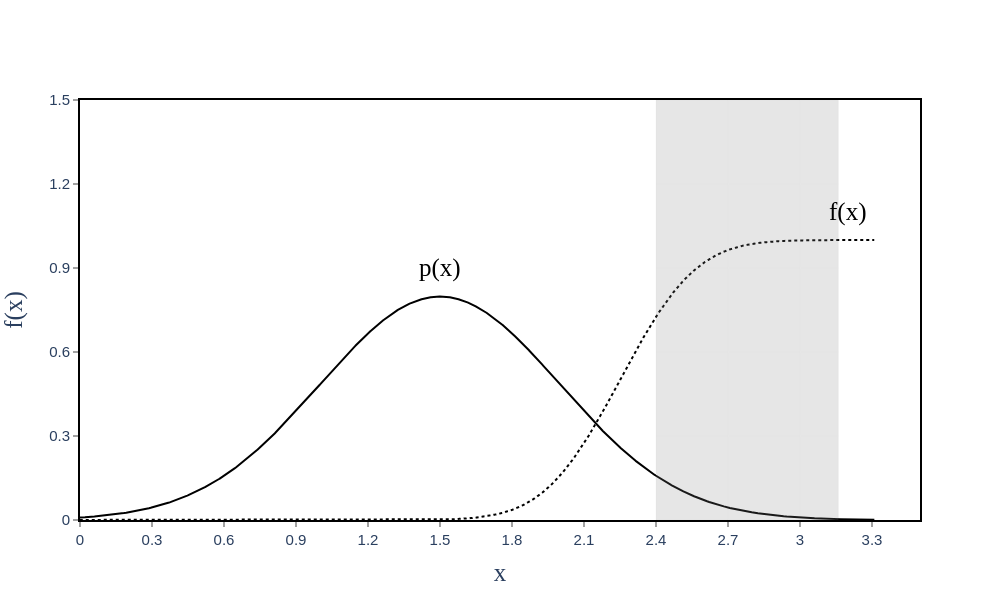
\includegraphics[scale=0.30]{Figures/Images/Illustrative Example/f&p.png}
        \caption{The graphs of $f(x)$ and $p(x)$ along with highlighted important region}
        \label{fig:f&p}
    \end{figure}

    As can be seen in Fig.~\ref{fig:f&p}, the \textit{important region} is highlighted on the graph, which is located in the tale of $p(x)$ with a very low probability of occurrence. 
    
    The goal here is to determine the expectation of f(x), which can be represented mathematically as:
    $$ E[f(x)]=\int f(x)p(x)dx $$
    For this specific example, it's easy to determine the expectation of $f(x)$ since it's a 1-dimensional problem and $ E[f(x)] $ can be easily calculated as the area under the $f(x)p(x)$ graph. The true value for this example is calculated as 0.087, shown in Fig.~\ref{fig:true_value}.
    
        \begin{figure}[H]
        \centering
        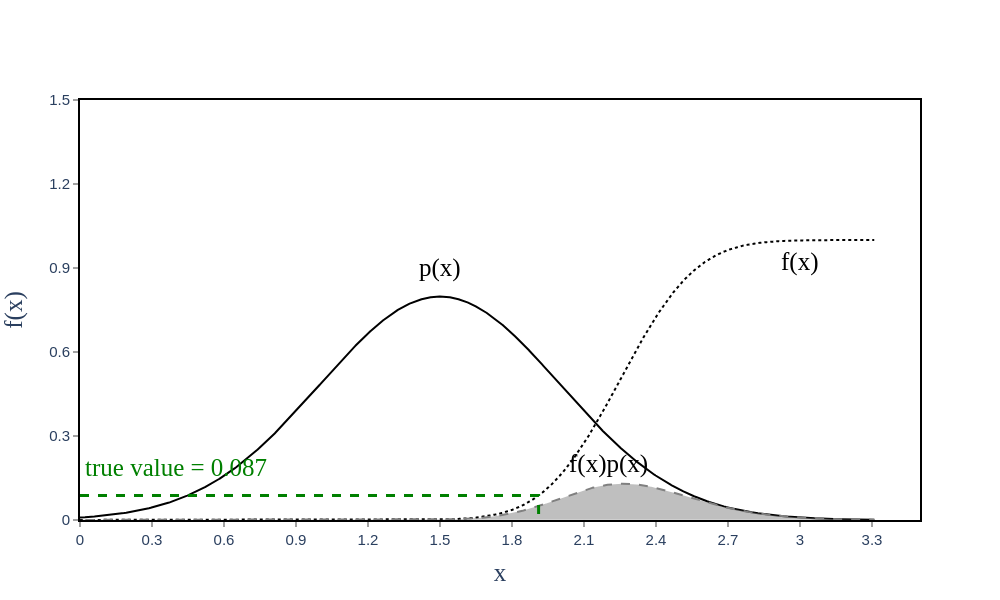
\includegraphics[scale=0.30]{Figures/Images/Illustrative Example/true_value.png}
        \caption{Calculation of the true value for the $E[f(x)]$}
        \label{fig:true_value}
    \end{figure}
    
    However, due to the high dimension of $x$, it is often impossible or very difficult to calculate the above integral analytically. As mentioned earlier, one of the most popular techniques that numerically approximates the expectation using an average is the Monte Carlo method, which can be expressed as follows:
    $$E[f(x)] \approx \frac{1}{N}\sum_{i=1}^{N} f(x) \quad \text{and} \quad x_i\sim p(x)$$  
    
    To estimate $E[f(x)]$ using the crude Monte Carlo method, we first sample $x’s$ from $p(x)$ and then plug those into $f(x)$. The average of these is an approximation of the expected value. This process is shown in Fig.~\ref{fig:crude_MC} with 20 samples. The number of samples is kept small due to the simplicity of this problem. \\

        \begin{figure}[H]
        \centering
        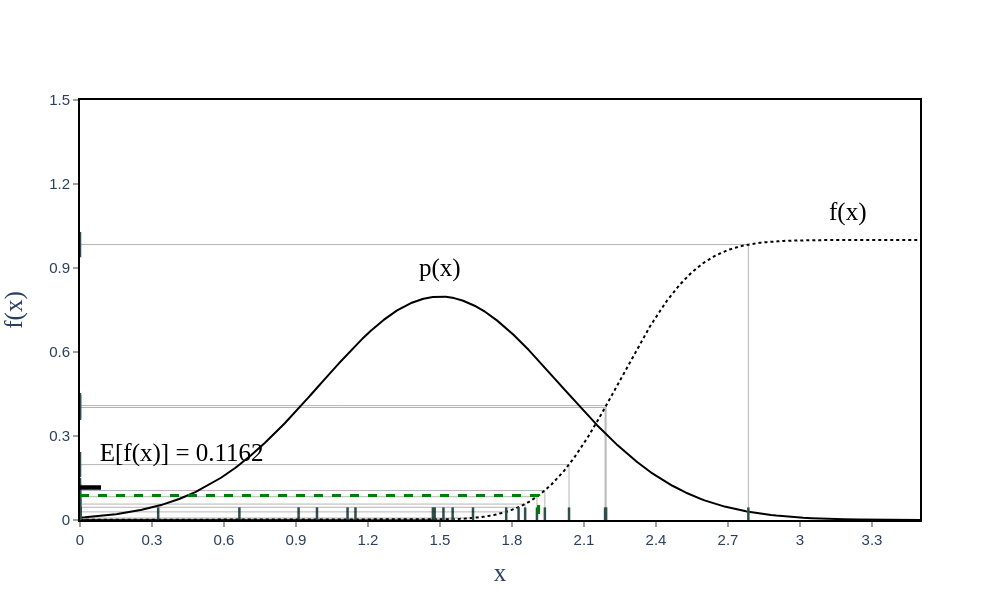
\includegraphics[scale=0.30]{Figures/Images/Illustrative Example/crude_MC.png}
        \caption{Crude Monte Carlo samples along with the estimation ($E[f(x)]$)}
        \label{fig:crude_MC}
    \end{figure}
    
    % When dealing with natural hazards, one may be only interested in worst-case samples which in this case are located in the tale of the $p(x)$. To test this approach, samples are generated from the truncated $p(x)$ where $x\geq 2.5$. The implementation of this method with 20 samples is shown in Fig.~\ref{fig:truncated_MC}. 
    
    %     \begin{figure}[H]
        \centering
        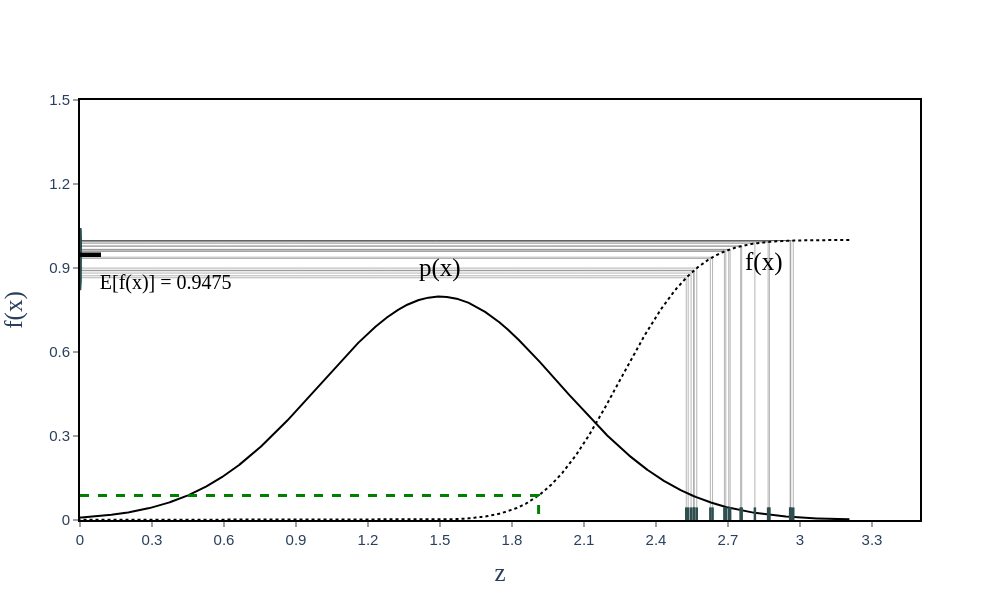
\includegraphics[scale=0.30]{Figures/Images/Illustrative Example/truncated_MC.png}
        \caption{Generated samples using crude Monte Carlo method from the truncated distribution function and the calculated $E[f(x)]$}
        \label{fig:truncated_MC}
    \end{figure}

    % For this implementation, the expectation of $f(x)$ is estimated to be 0.9475, and it can be shown that even with a very large sample size, the expectation value would still be close to 0.94 which is far from the actual expectation value (0.087).\\
    
    To implement the importance sampling method, a new probability distribution, $q(x)$, is required as the importance density function. As mentioned earlier, the traditional way to choose the important density function is to keep the family of the distribution the same as the original distribution but change the parameters. For this one-dimensional problem, it is evident that the mean value of the original distribution $p(x)$ should be shifted to the right in order to generate more important samples more frequently. To correct the generated bias, the $f(x)$ must be adjusted with a weighting factor equal to $\frac{p(x)}{q(x)}$. The importance distribution along with the 20 generated samples from the IS method are shown in Fig.~\ref{fig:IS_dist}.
    
        \begin{figure}[H]
        \centering
        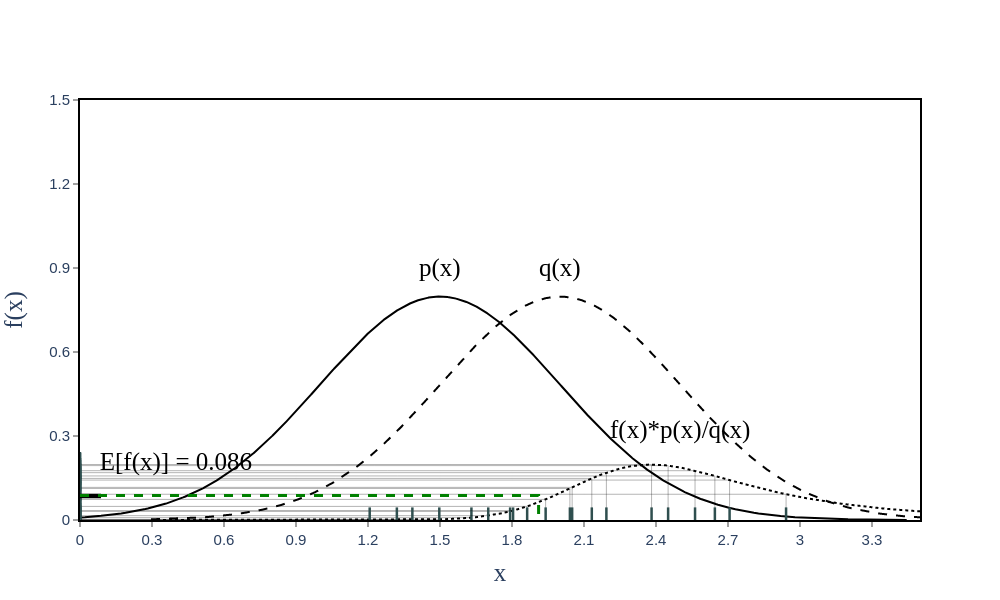
\includegraphics[scale=0.30]{Figures/Images/Illustrative Example/IS_dist.png}
        \caption{Importance sampling distribution along with generated samples and the calculated $E[f(x)]$}
        \label{fig:IS_dist}
    \end{figure}
    
    Although a variety of distributions can be employed as an importance density function, there is an optimal importance density that can generate MC estimates with no variance \cite{asmussen_stochastic_2007}. The mathematical expression of the optimum importance density function is as follows:
    $$q^*=\frac{f(x)p(x)}{\int f(x)p(x)dx}$$
    Where $q^{*}$ is the optimum importance density function.
    
    Because of the unknown value of $\int{f(x)}{p(x)}dx$, the above expression cannot be directly determined in practice. However, for this example, since we know the actual value of the integral, we can determine the optimum importance density, shown in Fig.~\ref{fig:opt_IS_dist}.

        \begin{figure}[H]
        \centering
        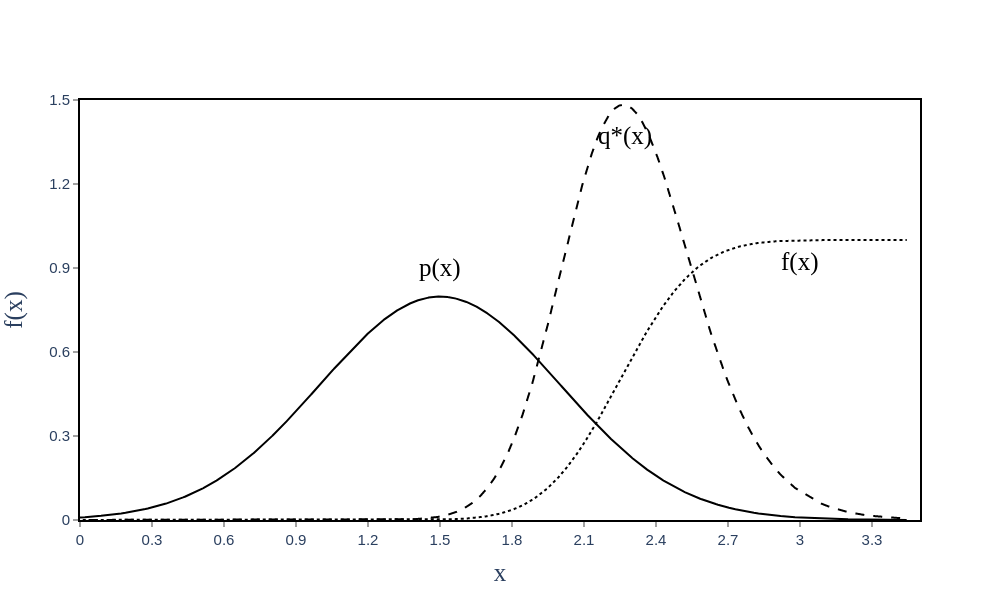
\includegraphics[scale=0.30]{Figures/Images/Illustrative Example/opt_IS_dist.png}
        \caption{Original probability distribution along with the optimum importance density function}
        \label{fig:opt_IS_dist}
    \end{figure}

    Although it is often difficult or impossible to determine the optimum importance density function, there are techniques to estimate the near-optimal importance density function. One of these techniques is MCMC-IS, which was previously described. This method generates samples from the Markov Chain Monte Carlo method, and the KDE fitted to those samples is considered the importance density function. The approximate importance density function from the MCMC-IS technique and the optimum importance density function is shown in Fig.~\ref{fig:opt_IS_dist}.

        \begin{figure}[H]
        \centering
        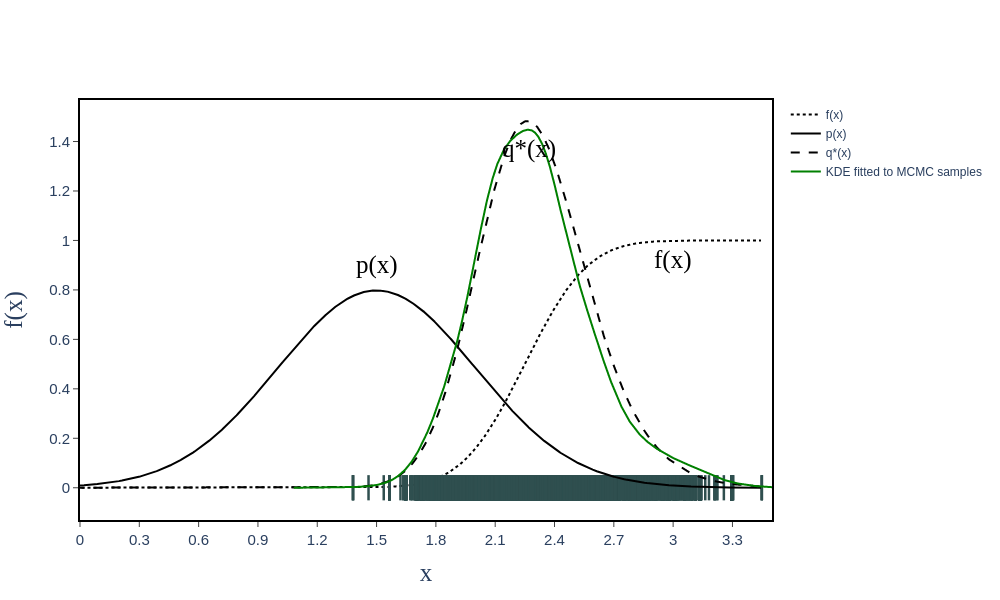
\includegraphics[scale=0.30]{Figures/Images/Illustrative Example/near_opt_IS_dist.png}
        \caption{Approximating the near-optimal importance sampling density function using MCMC-IS technique}
        \label{fig:near_opt_IS_dist}
    \end{figure}
    
    The KDE fitted to the MCMC samples shown in Fig.~\ref{fig:near_opt_IS_dist} is for 10000 MCMC samples and has a bandwidth of 0.1. However, the importance distribution resulting from MCMC-IS does not always perfectly match the optimum importance density function (as shown in Fig.~\ref{fig:opt_IS_dist}). There are two possible sources of error with this method. The first one is about MCMC samples, and the second one is about how the KDE fits to the MCMC samples. The number of samples created by the MCMC algorithm should be large enough, and the bandwidth parameter of the KDE algorithm should be small enough to control the error caused by the KDE algorithm. The approximation of the optimum importance density function using the MCMC-IS method for different MCMC sample sizes and KDE bandwidths are shown in Fig.~\ref{fig:near_opt_IS_dists}.\\

        \begin{figure}[H]
        \centering
        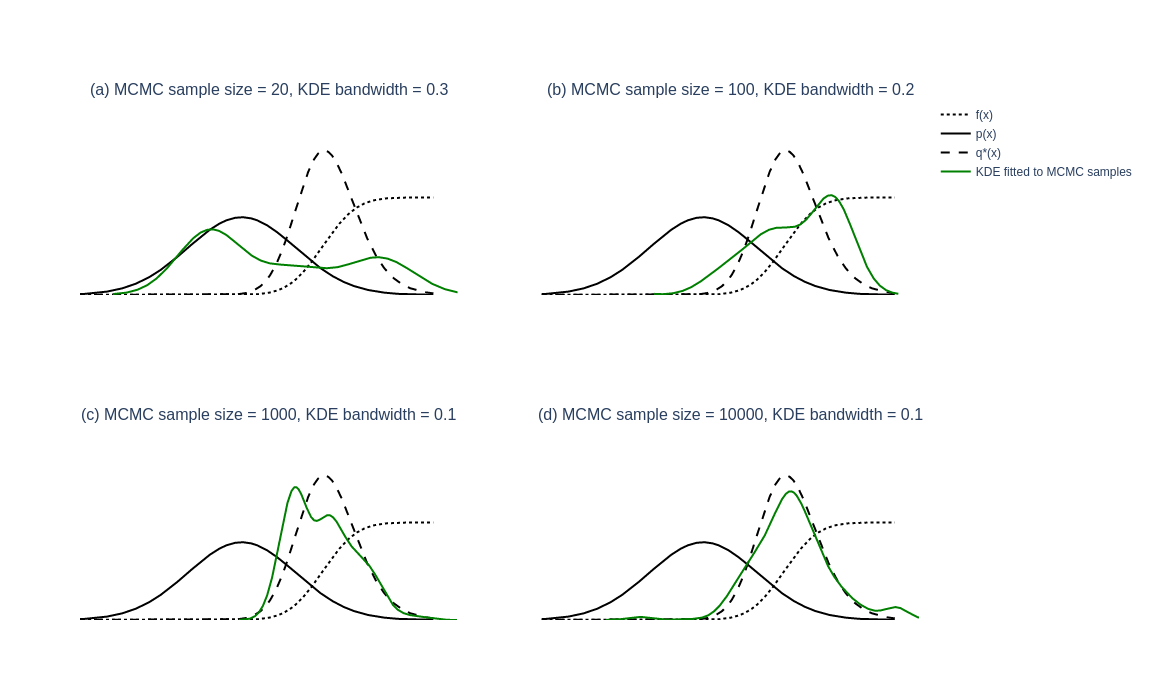
\includegraphics[scale=0.30]{Figures/Images/Illustrative Example/near_opt_IS_dists.png}
        \caption{The impacts of the MCMC number of samples and the KDE bandwidth on the approximation of the optimal importance density function}
        \label{fig:near_opt_IS_dists}
    \end{figure}

    As seen in Fig.~\ref{fig:near_opt_IS_dists}, more MCMC sample size and smaller KDE bandwidth will lead to a better estimate of the importance density function. 
    
    It is now necessary to compare the performance of the four aforementioned estimators. The following list of criteria can be used to evaluate how well various estimators perform. Having good qualities in balance is typically regarded as a criterion for assessing an estimator.
    \begin{itemize}[leftmargin=*]
      \item Bias\\
        The bias of an estimator is the difference between the estimator's expected value and the true value of the parameter being estimated. An estimator with zero bias is called an unbiased estimator.
        $$
        Bias(\widehat{f}(x))=E[f(x)]-\text{true value}
        $$
        where $\widehat{f}(x)$ is the estimation of $f(x)$.
      \item Finite sample variance\\
      The variance of estimation is the expected value of the squared sampling deviations: 
        $$
        Var(\widehat{f}(x))=E[\widehat{f}(x)-(E[\widehat{f}(x)])^2]
        $$
      \item Mean Square Error\\
        The mean squared error (MSE) is defined as the expected value (probability-weighted average, over all samples) of the squared errors ($E[(\widehat{f}(x)-\text{true value})^{2}]$) and it can be calculated as follows: 
        $$ 
        MSE(\widehat{f}(x))=Var(\widehat{f}(x))+Bias(\widehat{f}(x))^{2}
        $$
        MSE is the best criterion to evaluate a biased estimator.
        \item Consistency\\
        It turns out that many useful estimators are biased given the limited amount of data available. But one important criterion is that as we add more and more data, our estimator should usually get closer and closer to the right answer.
    \end{itemize}

    The variance, bias, and MSE for each suggested estimator for the sample size of 10 are listed in able.~\ref{table:illustrative_results_10}. It should be noted that, in the MCMC\_IS method, the KDE bandwidth is set to 0.1 and the number of MCMC samples is assumed to be 10,000.

    \begin{table}[H]
    \centering
    \caption{Comparison of the estimation, variance, and MSE produced by the three estimators with the sample size of 10 for the illustrative example}
    \label{table:illustrative_results_10}
    \small
    \begin{tabular}{lccc}
        \hline
        & \textbf{crude MC} & \textbf{Traditional IS} & \textbf{MCMC IS} \\
        \hline
        \textbf{Estimation}\\
        true value = 0.87 & 7.527e-2 & 8.791e-2 & 8.972e-2\\
        \textbf{Variance} & 3.052e-3 & 5.641e-4 & 3.189e-6\\
        \textbf{Mean Square Error (MSE)} & 3.200e-3 & 5.643e-4 & 8.344e-6\\
        \hline
    \end{tabular}
\end{table}
    \begin{table}[H]
    \centering
    \caption{Evaluation of the three estimators for the sample size of 100}
    \label{table:illustrative_results_100}
    \small
    \begin{tabular}{lccc}
        \hline
        & \textbf{crude MC} & \textbf{Traditional IS} & \textbf{MCMC IS} \\ 
            \hline
        \textbf{Estimation}\\
        true value = 0.87 & 9.091e-2 & 8.948e-2 & 8.979e-2\\
        \textbf{Variance} & 4.390e-4 & 5.569e-5 & 8.687e-7\\
        \textbf{Mean Square Error (MSE)} & 4.510e-4 & 5.981e-5 & 6.373e-6\\
        \hline
    \end{tabular}
\end{table}

    Table.~\ref{table:illustrative_results_10} shows that, among the three methods, MCMC-IS has the lowest MSE and variance, while crude-MC has the highest. \\
    Also, in order to compare the convergence rate of the three estimators, the estimation, variance, and MSE of the three estimators for different sample sizes are illustrated in Fig.~\ref{fig:running_properties}.\\

        \begin{figure}[H]
        \centering
        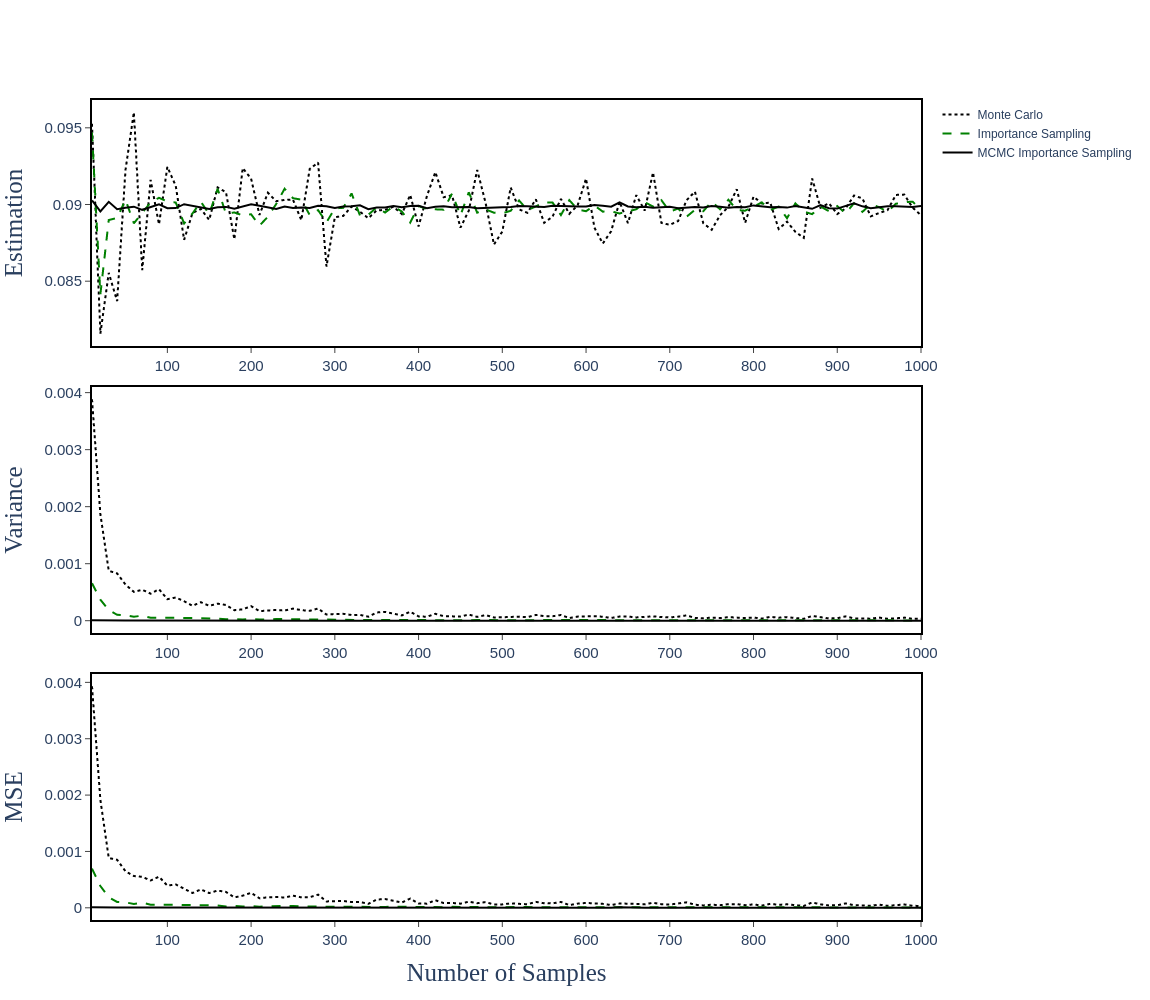
\includegraphics[scale=0.30]{Figures/Images/Illustrative Example/running_properties.png}
        \caption{Comparison of the estimation, variance, and MSE produced by the three estimators for illustrative example}
        \label{fig:running_properties}
    \end{figure}
    

    
        
        
